\documentclass[1p]{elsarticle_modified}
%\bibliographystyle{elsarticle-num}

%\usepackage[colorlinks]{hyperref}
%\usepackage{abbrmath_seonhwa} %\Abb, \Ascr, \Acal ,\Abf, \Afrak
\usepackage{amsfonts}
\usepackage{amssymb}
\usepackage{amsmath}
\usepackage{amsthm}
\usepackage{scalefnt}
\usepackage{amsbsy}
\usepackage{kotex}
\usepackage{caption}
\usepackage{subfig}
\usepackage{color}
\usepackage{graphicx}
\usepackage{xcolor} %% white, black, red, green, blue, cyan, magenta, yellow
\usepackage{float}
\usepackage{setspace}
\usepackage{hyperref}

\usepackage{tikz}
\usetikzlibrary{arrows}

\usepackage{multirow}
\usepackage{array} % fixed length table
\usepackage{hhline}

%%%%%%%%%%%%%%%%%%%%%
\makeatletter
\renewcommand*\env@matrix[1][\arraystretch]{%
	\edef\arraystretch{#1}%
	\hskip -\arraycolsep
	\let\@ifnextchar\new@ifnextchar
	\array{*\c@MaxMatrixCols c}}
\makeatother %https://tex.stackexchange.com/questions/14071/how-can-i-increase-the-line-spacing-in-a-matrix
%%%%%%%%%%%%%%%

\usepackage[normalem]{ulem}

\newcommand{\msout}[1]{\ifmmode\text{\sout{\ensuremath{#1}}}\else\sout{#1}\fi}
%SOURCE: \msout is \stkout macro in https://tex.stackexchange.com/questions/20609/strikeout-in-math-mode

\newcommand{\cancel}[1]{
	\ifmmode
	{\color{red}\msout{#1}}
	\else
	{\color{red}\sout{#1}}
	\fi
}

\newcommand{\add}[1]{
	{\color{blue}\uwave{#1}}
}

\newcommand{\replace}[2]{
	\ifmmode
	{\color{red}\msout{#1}}{\color{blue}\uwave{#2}}
	\else
	{\color{red}\sout{#1}}{\color{blue}\uwave{#2}}
	\fi
}

\newcommand{\Sol}{\mathcal{S}} %segment
\newcommand{\D}{D} %diagram
\newcommand{\A}{\mathcal{A}} %arc


%%%%%%%%%%%%%%%%%%%%%%%%%%%%%5 test

\def\sl{\operatorname{\textup{SL}}(2,\Cbb)}
\def\psl{\operatorname{\textup{PSL}}(2,\Cbb)}
\def\quan{\mkern 1mu \triangleright \mkern 1mu}

\theoremstyle{definition}
\newtheorem{thm}{Theorem}[section]
\newtheorem{prop}[thm]{Proposition}
\newtheorem{lem}[thm]{Lemma}
\newtheorem{ques}[thm]{Question}
\newtheorem{cor}[thm]{Corollary}
\newtheorem{defn}[thm]{Definition}
\newtheorem{exam}[thm]{Example}
\newtheorem{rmk}[thm]{Remark}
\newtheorem{alg}[thm]{Algorithm}

\newcommand{\I}{\sqrt{-1}}
\begin{document}

%\begin{frontmatter}
%
%\title{Boundary parabolic representations of knots up to 8 crossings}
%
%%% Group authors per affiliation:
%\author{Yunhi Cho} 
%\address{Department of Mathematics, University of Seoul, Seoul, Korea}
%\ead{yhcho@uos.ac.kr}
%
%
%\author{Seonhwa Kim} %\fnref{s_kim}}
%\address{Center for Geometry and Physics, Institute for Basic Science, Pohang, 37673, Korea}
%\ead{ryeona17@ibs.re.kr}
%
%\author{Hyuk Kim}
%\address{Department of Mathematical Sciences, Seoul National University, Seoul 08826, Korea}
%\ead{hyukkim@snu.ac.kr}
%
%\author{Seokbeom Yoon}
%\address{Department of Mathematical Sciences, Seoul National University, Seoul, 08826,  Korea}
%\ead{sbyoon15@snu.ac.kr}
%
%\begin{abstract}
%We find all boundary parabolic representation of knots up to 8 crossings.
%
%\end{abstract}
%\begin{keyword}
%    \MSC[2010] 57M25 
%\end{keyword}
%
%\end{frontmatter}

%\linenumbers
%\tableofcontents
%
\newcommand\colored[1]{\textcolor{white}{\rule[-0.35ex]{0.8em}{1.4ex}}\kern-0.8em\color{red} #1}%
%\newcommand\colored[1]{\textcolor{white}{ #1}\kern-2.17ex	\textcolor{white}{ #1}\kern-1.81ex	\textcolor{white}{ #1}\kern-2.15ex\color{red}#1	}

{\Large $\underline{12n_{0234}~(K12n_{0234})}$}

\setlength{\tabcolsep}{10pt}
\renewcommand{\arraystretch}{1.6}
\vspace{1cm}\begin{tabular}{m{100pt}>{\centering\arraybackslash}m{274pt}}
\multirow{5}{120pt}{
	\centering
	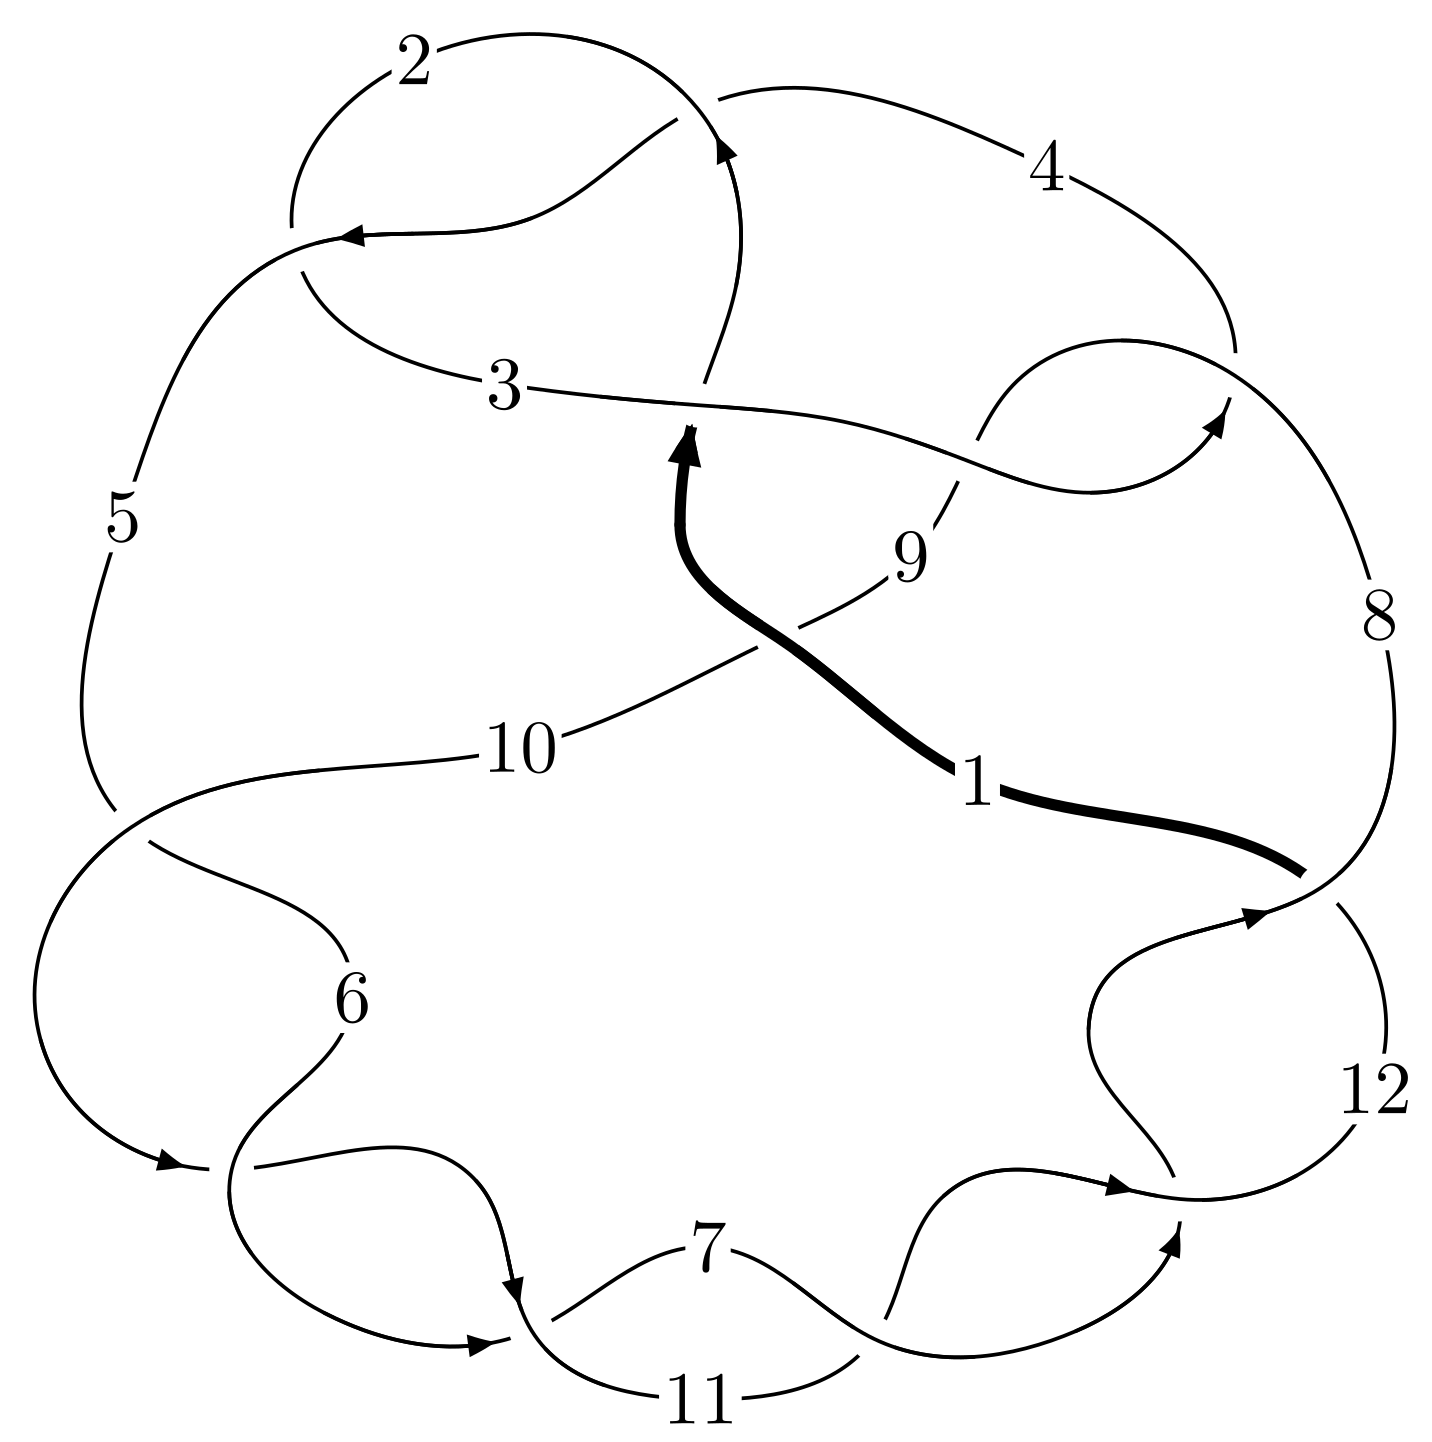
\includegraphics[width=112pt]{../../../GIT/diagram.site/Diagrams/png/2323_12n_0234.png}\\
\ \ \ A knot diagram\footnotemark}&
\allowdisplaybreaks
\textbf{Linearized knot diagam} \\
\cline{2-2}
 &
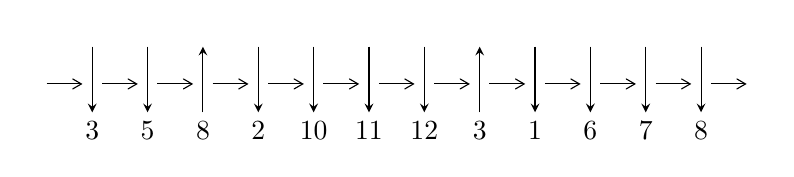
\begin{tikzpicture}[x=20pt, y=17pt]
	% nodes
	\node (C0) at (0, 0) {};
	\node (C1) at (1, 0) {};
	\node (C1U) at (1, +1) {};
	\node (C1D) at (1, -1) {3};

	\node (C2) at (2, 0) {};
	\node (C2U) at (2, +1) {};
	\node (C2D) at (2, -1) {5};

	\node (C3) at (3, 0) {};
	\node (C3U) at (3, +1) {};
	\node (C3D) at (3, -1) {8};

	\node (C4) at (4, 0) {};
	\node (C4U) at (4, +1) {};
	\node (C4D) at (4, -1) {2};

	\node (C5) at (5, 0) {};
	\node (C5U) at (5, +1) {};
	\node (C5D) at (5, -1) {10};

	\node (C6) at (6, 0) {};
	\node (C6U) at (6, +1) {};
	\node (C6D) at (6, -1) {11};

	\node (C7) at (7, 0) {};
	\node (C7U) at (7, +1) {};
	\node (C7D) at (7, -1) {12};

	\node (C8) at (8, 0) {};
	\node (C8U) at (8, +1) {};
	\node (C8D) at (8, -1) {3};

	\node (C9) at (9, 0) {};
	\node (C9U) at (9, +1) {};
	\node (C9D) at (9, -1) {1};

	\node (C10) at (10, 0) {};
	\node (C10U) at (10, +1) {};
	\node (C10D) at (10, -1) {6};

	\node (C11) at (11, 0) {};
	\node (C11U) at (11, +1) {};
	\node (C11D) at (11, -1) {7};

	\node (C12) at (12, 0) {};
	\node (C12U) at (12, +1) {};
	\node (C12D) at (12, -1) {8};
	\node (C13) at (13, 0) {};

	% arrows
	\draw[->,>={angle 60}]
	(C0) edge (C1) (C1) edge (C2) (C2) edge (C3) (C3) edge (C4) (C4) edge (C5) (C5) edge (C6) (C6) edge (C7) (C7) edge (C8) (C8) edge (C9) (C9) edge (C10) (C10) edge (C11) (C11) edge (C12) (C12) edge (C13) ;	\draw[->,>=stealth]
	(C1U) edge (C1D) (C2U) edge (C2D) (C3D) edge (C3U) (C4U) edge (C4D) (C5U) edge (C5D) (C6U) edge (C6D) (C7U) edge (C7D) (C8D) edge (C8U) (C9U) edge (C9D) (C10U) edge (C10D) (C11U) edge (C11D) (C12U) edge (C12D) ;
	\end{tikzpicture} \\
\hhline{~~} \\& 
\textbf{Solving Sequence} \\ \cline{2-2} 
 &
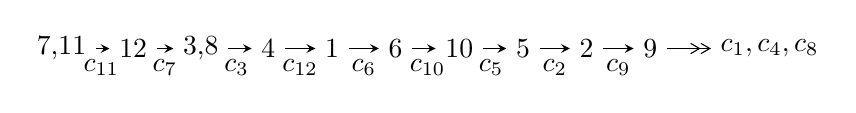
\begin{tikzpicture}[x=23pt, y=7pt]
	% node
	\node (A0) at (-1/8, 0) {7,11};
	\node (A1) at (1, 0) {12};
	\node (A2) at (33/16, 0) {3,8};
	\node (A3) at (25/8, 0) {4};
	\node (A4) at (33/8, 0) {1};
	\node (A5) at (41/8, 0) {6};
	\node (A6) at (49/8, 0) {10};
	\node (A7) at (57/8, 0) {5};
	\node (A8) at (65/8, 0) {2};
	\node (A9) at (73/8, 0) {9};
	\node (C1) at (1/2, -1) {$c_{11}$};
	\node (C2) at (3/2, -1) {$c_{7}$};
	\node (C3) at (21/8, -1) {$c_{3}$};
	\node (C4) at (29/8, -1) {$c_{12}$};
	\node (C5) at (37/8, -1) {$c_{6}$};
	\node (C6) at (45/8, -1) {$c_{10}$};
	\node (C7) at (53/8, -1) {$c_{5}$};
	\node (C8) at (61/8, -1) {$c_{2}$};
	\node (C9) at (69/8, -1) {$c_{9}$};
	\node (A10) at (11, 0) {$c_{1},c_{4},c_{8}$};

	% edge
	\draw[->,>=stealth]	
	(A0) edge (A1) (A1) edge (A2) (A2) edge (A3) (A3) edge (A4) (A4) edge (A5) (A5) edge (A6) (A6) edge (A7) (A7) edge (A8) (A8) edge (A9) ;
	\draw[->>,>={angle 60}]	
	(A9) edge (A10);
\end{tikzpicture} \\ 

\end{tabular} \\

\footnotetext{
The image of knot diagram is generated by the software ``\textbf{Draw programme}" developed by Andrew Bartholomew(\url{http://www.layer8.co.uk/maths/draw/index.htm\#Running-draw}), where we modified some parts for our purpose(\url{https://github.com/CATsTAILs/LinksPainter}).
}\phantom \\ \newline 
\centering \textbf{Ideals for irreducible components\footnotemark of $X_{\text{par}}$} 
 
\begin{align*}
I^u_{1}&=\langle 
- u^{23}+16 u^{21}+\cdots+b-1,\;- u^{22}+15 u^{20}+\cdots+a+1,\;u^{24}-2 u^{23}+\cdots+u-1\rangle \\
I^u_{2}&=\langle 
u^2+b-1,\;a+1,\;u^3+u^2-2 u-1\rangle \\
\\
\end{align*}
\raggedright * 2 irreducible components of $\dim_{\mathbb{C}}=0$, with total 27 representations.\\
\footnotetext{All coefficients of polynomials are rational numbers. But the coefficients are sometimes approximated in decimal forms when there is not enough margin.}
\newpage
\renewcommand{\arraystretch}{1}
\centering \section*{I. $I^u_{1}= \langle - u^{23}+16 u^{21}+\cdots+b-1,\;- u^{22}+15 u^{20}+\cdots+a+1,\;u^{24}-2 u^{23}+\cdots+u-1 \rangle$}
\flushleft \textbf{(i) Arc colorings}\\
\begin{tabular}{m{7pt} m{180pt} m{7pt} m{180pt} }
\flushright $a_{7}=$&$\begin{pmatrix}0\\u\end{pmatrix}$ \\
\flushright $a_{11}=$&$\begin{pmatrix}1\\0\end{pmatrix}$ \\
\flushright $a_{12}=$&$\begin{pmatrix}1\\u^2\end{pmatrix}$ \\
\flushright $a_{3}=$&$\begin{pmatrix}u^{22}-15 u^{20}+\cdots-6 u-1\\u^{23}-16 u^{21}+\cdots+u+1\end{pmatrix}$ \\
\flushright $a_{8}=$&$\begin{pmatrix}- u\\- u^3+u\end{pmatrix}$ \\
\flushright $a_{4}=$&$\begin{pmatrix}-2 u^{23}+2 u^{22}+\cdots-6 u-2\\-3 u^{23}+u^{22}+\cdots+2 u-1\end{pmatrix}$ \\
\flushright $a_{1}=$&$\begin{pmatrix}- u^2+1\\- u^4+2 u^2\end{pmatrix}$ \\
\flushright $a_{6}=$&$\begin{pmatrix}u\\u\end{pmatrix}$ \\
\flushright $a_{10}=$&$\begin{pmatrix}- u^2+1\\- u^2\end{pmatrix}$ \\
\flushright $a_{5}=$&$\begin{pmatrix}- u^3+2 u\\- u^3+u\end{pmatrix}$ \\
\flushright $a_{2}=$&$\begin{pmatrix}- u^{23}+u^{22}+\cdots-5 u-1\\- u^{23}+15 u^{21}+\cdots+8 u^2+2 u\end{pmatrix}$ \\
\flushright $a_{9}=$&$\begin{pmatrix}u^8-5 u^6+7 u^4-4 u^2+1\\u^{10}-6 u^8+11 u^6-6 u^4- u^2\end{pmatrix}$\\&\end{tabular}
\flushleft \textbf{(ii) Obstruction class $= -1$}\\~\\
\flushleft \textbf{(iii) Cusp Shapes $= u^{23}-4 u^{22}-16 u^{21}+62 u^{20}+110 u^{19}-405 u^{18}-420 u^{17}+1453 u^{16}+940 u^{15}-3134 u^{14}-1118 u^{13}+4197 u^{12}+260 u^{11}-3495 u^{10}+1034 u^9+1741 u^8-1269 u^7-400 u^6+550 u^5-66 u^4-92 u^3+43 u^2+22 u-5$}\\~\\
\newpage\renewcommand{\arraystretch}{1}
\flushleft \textbf{(iv) u-Polynomials at the component}\newline \\
\begin{tabular}{m{50pt}|m{274pt}}
Crossings & \hspace{64pt}u-Polynomials at each crossing \\
\hline $$\begin{aligned}c_{1}\end{aligned}$$&$\begin{aligned}
&u^{24}+8 u^{23}+\cdots+34 u+1
\end{aligned}$\\
\hline $$\begin{aligned}c_{2},c_{4}\end{aligned}$$&$\begin{aligned}
&u^{24}-4 u^{23}+\cdots+6 u-1
\end{aligned}$\\
\hline $$\begin{aligned}c_{3},c_{8}\end{aligned}$$&$\begin{aligned}
&u^{24}+u^{23}+\cdots+36 u+8
\end{aligned}$\\
\hline $$\begin{aligned}c_{5},c_{6},c_{7}\\c_{10},c_{11},c_{12}\end{aligned}$$&$\begin{aligned}
&u^{24}-2 u^{23}+\cdots+u-1
\end{aligned}$\\
\hline $$\begin{aligned}c_{9}\end{aligned}$$&$\begin{aligned}
&u^{24}+2 u^{23}+\cdots+7 u+1
\end{aligned}$\\
\hline
\end{tabular}\\~\\
\newpage\renewcommand{\arraystretch}{1}
\flushleft \textbf{(v) Riley Polynomials at the component}\newline \\
\begin{tabular}{m{50pt}|m{274pt}}
Crossings & \hspace{64pt}Riley Polynomials at each crossing \\
\hline $$\begin{aligned}c_{1}\end{aligned}$$&$\begin{aligned}
&y^{24}+20 y^{23}+\cdots-534 y+1
\end{aligned}$\\
\hline $$\begin{aligned}c_{2},c_{4}\end{aligned}$$&$\begin{aligned}
&y^{24}-8 y^{23}+\cdots-34 y+1
\end{aligned}$\\
\hline $$\begin{aligned}c_{3},c_{8}\end{aligned}$$&$\begin{aligned}
&y^{24}-21 y^{23}+\cdots-1040 y+64
\end{aligned}$\\
\hline $$\begin{aligned}c_{5},c_{6},c_{7}\\c_{10},c_{11},c_{12}\end{aligned}$$&$\begin{aligned}
&y^{24}-34 y^{23}+\cdots-21 y+1
\end{aligned}$\\
\hline $$\begin{aligned}c_{9}\end{aligned}$$&$\begin{aligned}
&y^{24}+26 y^{23}+\cdots-21 y+1
\end{aligned}$\\
\hline
\end{tabular}\\~\\
\newpage\flushleft \textbf{(vi) Complex Volumes and Cusp Shapes}
$$\begin{array}{c|c|c}  
\text{Solutions to }I^u_{1}& \I (\text{vol} + \sqrt{-1}CS) & \text{Cusp shape}\\
 \hline 
\begin{aligned}
u &= \phantom{-}1.065440 + 0.105091 I \\
a &= -0.101056 - 1.017940 I \\
b &= \phantom{-}0.427572 + 0.787716 I\end{aligned}
 & -4.78298 - 2.15986 I & -14.8245 + 3.7042 I \\ \hline\begin{aligned}
u &= \phantom{-}1.065440 - 0.105091 I \\
a &= -0.101056 + 1.017940 I \\
b &= \phantom{-}0.427572 - 0.787716 I\end{aligned}
 & -4.78298 + 2.15986 I & -14.8245 - 3.7042 I \\ \hline\begin{aligned}
u &= -1.044560 + 0.293303 I \\
a &= \phantom{-}0.060787 - 0.485482 I \\
b &= \phantom{-}0.951447 + 0.437799 I\end{aligned}
 & \phantom{-}0.73559 + 1.57187 I & -10.92931 - 1.48898 I \\ \hline\begin{aligned}
u &= -1.044560 - 0.293303 I \\
a &= \phantom{-}0.060787 + 0.485482 I \\
b &= \phantom{-}0.951447 - 0.437799 I\end{aligned}
 & \phantom{-}0.73559 - 1.57187 I & -10.92931 + 1.48898 I \\ \hline\begin{aligned}
u &= -1.08841\phantom{ +0.000000I} \\
a &= -1.48671\phantom{ +0.000000I} \\
b &= -1.10653\phantom{ +0.000000I}\end{aligned}
 & -6.35267\phantom{ +0.000000I} & -13.5900\phantom{ +0.000000I} \\ \hline\begin{aligned}
u &= -1.158950 + 0.291958 I \\
a &= \phantom{-}0.215884 + 1.148480 I \\
b &= -0.234965 - 0.552300 I\end{aligned}
 & -0.44591 + 7.86280 I & -12.55352 - 5.99165 I \\ \hline\begin{aligned}
u &= -1.158950 - 0.291958 I \\
a &= \phantom{-}0.215884 - 1.148480 I \\
b &= -0.234965 + 0.552300 I\end{aligned}
 & -0.44591 - 7.86280 I & -12.55352 + 5.99165 I \\ \hline\begin{aligned}
u &= \phantom{-}1.29716\phantom{ +0.000000I} \\
a &= -0.674636\phantom{ +0.000000I} \\
b &= \phantom{-}0.0175724\phantom{ +0.000000I}\end{aligned}
 & -7.12889\phantom{ +0.000000I} & -9.59420\phantom{ +0.000000I} \\ \hline\begin{aligned}
u &= \phantom{-}0.413733 + 0.547171 I \\
a &= -0.390896 + 1.056560 I \\
b &= -0.969122 + 0.621169 I\end{aligned}
 & \phantom{-}4.52862 - 4.98340 I & -8.25902 + 6.13145 I \\ \hline\begin{aligned}
u &= \phantom{-}0.413733 - 0.547171 I \\
a &= -0.390896 - 1.056560 I \\
b &= -0.969122 - 0.621169 I\end{aligned}
 & \phantom{-}4.52862 + 4.98340 I & -8.25902 - 6.13145 I\\
 \hline 
 \end{array}$$\newpage$$\begin{array}{c|c|c}  
\text{Solutions to }I^u_{1}& \I (\text{vol} + \sqrt{-1}CS) & \text{Cusp shape}\\
 \hline 
\begin{aligned}
u &= \phantom{-}0.292302 + 0.564711 I \\
a &= \phantom{-}0.90790 - 1.36582 I \\
b &= \phantom{-}0.567413 + 0.008562 I\end{aligned}
 & \phantom{-}4.89005 + 1.34187 I & -6.87930 + 0.47018 I \\ \hline\begin{aligned}
u &= \phantom{-}0.292302 - 0.564711 I \\
a &= \phantom{-}0.90790 + 1.36582 I \\
b &= \phantom{-}0.567413 - 0.008562 I\end{aligned}
 & \phantom{-}4.89005 - 1.34187 I & -6.87930 - 0.47018 I \\ \hline\begin{aligned}
u &= -0.544664\phantom{ +0.000000I} \\
a &= \phantom{-}0.533142\phantom{ +0.000000I} \\
b &= \phantom{-}0.444791\phantom{ +0.000000I}\end{aligned}
 & -0.910827\phantom{ +0.000000I} & -10.5330\phantom{ +0.000000I} \\ \hline\begin{aligned}
u &= -0.260496 + 0.277785 I \\
a &= \phantom{-}1.25655 - 0.85026 I \\
b &= -0.092184 - 0.632306 I\end{aligned}
 & -0.635329 + 0.918549 I & -9.38568 - 7.31949 I \\ \hline\begin{aligned}
u &= -0.260496 - 0.277785 I \\
a &= \phantom{-}1.25655 + 0.85026 I \\
b &= -0.092184 + 0.632306 I\end{aligned}
 & -0.635329 - 0.918549 I & -9.38568 + 7.31949 I \\ \hline\begin{aligned}
u &= \phantom{-}0.266177\phantom{ +0.000000I} \\
a &= -2.54350\phantom{ +0.000000I} \\
b &= \phantom{-}0.862360\phantom{ +0.000000I}\end{aligned}
 & -2.02344\phantom{ +0.000000I} & \phantom{-}2.35380\phantom{ +0.000000I} \\ \hline\begin{aligned}
u &= \phantom{-}1.73483 + 0.06615 I \\
a &= -1.05402 + 1.43450 I \\
b &= -1.58632 + 2.38877 I\end{aligned}
 & -9.17857 - 2.99479 I & -11.67464 + 0.80624 I \\ \hline\begin{aligned}
u &= \phantom{-}1.73483 - 0.06615 I \\
a &= -1.05402 - 1.43450 I \\
b &= -1.58632 - 2.38877 I\end{aligned}
 & -9.17857 + 2.99479 I & -11.67464 - 0.80624 I \\ \hline\begin{aligned}
u &= -1.74821 + 0.02394 I \\
a &= -0.42595 + 2.65836 I \\
b &= -0.53152 + 4.79437 I\end{aligned}
 & -14.9721 + 2.6782 I & -14.7087 - 2.4859 I \\ \hline\begin{aligned}
u &= -1.74821 - 0.02394 I \\
a &= -0.42595 - 2.65836 I \\
b &= -0.53152 - 4.79437 I\end{aligned}
 & -14.9721 - 2.6782 I & -14.7087 + 2.4859 I\\
 \hline 
 \end{array}$$\newpage$$\begin{array}{c|c|c}  
\text{Solutions to }I^u_{1}& \I (\text{vol} + \sqrt{-1}CS) & \text{Cusp shape}\\
 \hline 
\begin{aligned}
u &= \phantom{-}1.75360\phantom{ +0.000000I} \\
a &= -0.586507\phantom{ +0.000000I} \\
b &= -1.87176\phantom{ +0.000000I}\end{aligned}
 & -16.6700\phantom{ +0.000000I} & -14.3680\phantom{ +0.000000I} \\ \hline\begin{aligned}
u &= \phantom{-}1.76989 + 0.07670 I \\
a &= \phantom{-}1.04117 - 2.39816 I \\
b &= \phantom{-}2.07334 - 4.41830 I\end{aligned}
 & -11.0119 - 9.4629 I & -13.6249 + 4.9785 I \\ \hline\begin{aligned}
u &= \phantom{-}1.76989 - 0.07670 I \\
a &= \phantom{-}1.04117 + 2.39816 I \\
b &= \phantom{-}2.07334 + 4.41830 I\end{aligned}
 & -11.0119 + 9.4629 I & -13.6249 - 4.9785 I \\ \hline\begin{aligned}
u &= -1.81183\phantom{ +0.000000I} \\
a &= -1.26255\phantom{ +0.000000I} \\
b &= -2.55776\phantom{ +0.000000I}\end{aligned}
 & -18.6696\phantom{ +0.000000I} & -7.58970\phantom{ +0.000000I}\\
 \hline 
 \end{array}$$\newpage\newpage\renewcommand{\arraystretch}{1}
\centering \section*{II. $I^u_{2}= \langle u^2+b-1,\;a+1,\;u^3+u^2-2 u-1 \rangle$}
\flushleft \textbf{(i) Arc colorings}\\
\begin{tabular}{m{7pt} m{180pt} m{7pt} m{180pt} }
\flushright $a_{7}=$&$\begin{pmatrix}0\\u\end{pmatrix}$ \\
\flushright $a_{11}=$&$\begin{pmatrix}1\\0\end{pmatrix}$ \\
\flushright $a_{12}=$&$\begin{pmatrix}1\\u^2\end{pmatrix}$ \\
\flushright $a_{3}=$&$\begin{pmatrix}-1\\- u^2+1\end{pmatrix}$ \\
\flushright $a_{8}=$&$\begin{pmatrix}- u\\u^2- u-1\end{pmatrix}$ \\
\flushright $a_{4}=$&$\begin{pmatrix}-1\\- u^2+1\end{pmatrix}$ \\
\flushright $a_{1}=$&$\begin{pmatrix}- u^2+1\\- u^2+u+1\end{pmatrix}$ \\
\flushright $a_{6}=$&$\begin{pmatrix}u\\u\end{pmatrix}$ \\
\flushright $a_{10}=$&$\begin{pmatrix}- u^2+1\\- u^2\end{pmatrix}$ \\
\flushright $a_{5}=$&$\begin{pmatrix}u^2-1\\u^2- u-1\end{pmatrix}$ \\
\flushright $a_{2}=$&$\begin{pmatrix}- u^2\\-2 u^2+u+2\end{pmatrix}$ \\
\flushright $a_{9}=$&$\begin{pmatrix}- u\\u^2- u-1\end{pmatrix}$\\&\end{tabular}
\flushleft \textbf{(ii) Obstruction class $= 1$}\\~\\
\flushleft \textbf{(iii) Cusp Shapes $= u^2+u-23$}\\~\\
\newpage\renewcommand{\arraystretch}{1}
\flushleft \textbf{(iv) u-Polynomials at the component}\newline \\
\begin{tabular}{m{50pt}|m{274pt}}
Crossings & \hspace{64pt}u-Polynomials at each crossing \\
\hline $$\begin{aligned}c_{1},c_{2}\end{aligned}$$&$\begin{aligned}
&(u-1)^3
\end{aligned}$\\
\hline $$\begin{aligned}c_{3},c_{8}\end{aligned}$$&$\begin{aligned}
&u^3
\end{aligned}$\\
\hline $$\begin{aligned}c_{4}\end{aligned}$$&$\begin{aligned}
&(u+1)^3
\end{aligned}$\\
\hline $$\begin{aligned}c_{5},c_{6},c_{7}\\c_{9}\end{aligned}$$&$\begin{aligned}
&u^3- u^2-2 u+1
\end{aligned}$\\
\hline $$\begin{aligned}c_{10},c_{11},c_{12}\end{aligned}$$&$\begin{aligned}
&u^3+u^2-2 u-1
\end{aligned}$\\
\hline
\end{tabular}\\~\\
\newpage\renewcommand{\arraystretch}{1}
\flushleft \textbf{(v) Riley Polynomials at the component}\newline \\
\begin{tabular}{m{50pt}|m{274pt}}
Crossings & \hspace{64pt}Riley Polynomials at each crossing \\
\hline $$\begin{aligned}c_{1},c_{2},c_{4}\end{aligned}$$&$\begin{aligned}
&(y-1)^3
\end{aligned}$\\
\hline $$\begin{aligned}c_{3},c_{8}\end{aligned}$$&$\begin{aligned}
&y^3
\end{aligned}$\\
\hline $$\begin{aligned}c_{5},c_{6},c_{7}\\c_{9},c_{10},c_{11}\\c_{12}\end{aligned}$$&$\begin{aligned}
&y^3-5 y^2+6 y-1
\end{aligned}$\\
\hline
\end{tabular}\\~\\
\newpage\flushleft \textbf{(vi) Complex Volumes and Cusp Shapes}
$$\begin{array}{c|c|c}  
\text{Solutions to }I^u_{2}& \I (\text{vol} + \sqrt{-1}CS) & \text{Cusp shape}\\
 \hline 
\begin{aligned}
u &= \phantom{-}1.24698\phantom{ +0.000000I} \\
a &= -1.00000\phantom{ +0.000000I} \\
b &= -0.554958\phantom{ +0.000000I}\end{aligned}
 & -7.98968\phantom{ +0.000000I} & -20.1980\phantom{ +0.000000I} \\ \hline\begin{aligned}
u &= -0.445042\phantom{ +0.000000I} \\
a &= -1.00000\phantom{ +0.000000I} \\
b &= \phantom{-}0.801938\phantom{ +0.000000I}\end{aligned}
 & -2.34991\phantom{ +0.000000I} & -23.2470\phantom{ +0.000000I} \\ \hline\begin{aligned}
u &= -1.80194\phantom{ +0.000000I} \\
a &= -1.00000\phantom{ +0.000000I} \\
b &= -2.24698\phantom{ +0.000000I}\end{aligned}
 & -19.2692\phantom{ +0.000000I} & -21.5550\phantom{ +0.000000I}\\
 \hline 
 \end{array}$$\newpage
\newpage\renewcommand{\arraystretch}{1}
\centering \section*{ III. u-Polynomials}
\begin{tabular}{m{50pt}|m{274pt}}
Crossings & \hspace{64pt}u-Polynomials at each crossing \\
\hline $$\begin{aligned}c_{1}\end{aligned}$$&$\begin{aligned}
&((u-1)^3)(u^{24}+8 u^{23}+\cdots+34 u+1)
\end{aligned}$\\
\hline $$\begin{aligned}c_{2}\end{aligned}$$&$\begin{aligned}
&((u-1)^3)(u^{24}-4 u^{23}+\cdots+6 u-1)
\end{aligned}$\\
\hline $$\begin{aligned}c_{3},c_{8}\end{aligned}$$&$\begin{aligned}
&u^3(u^{24}+u^{23}+\cdots+36 u+8)
\end{aligned}$\\
\hline $$\begin{aligned}c_{4}\end{aligned}$$&$\begin{aligned}
&((u+1)^3)(u^{24}-4 u^{23}+\cdots+6 u-1)
\end{aligned}$\\
\hline $$\begin{aligned}c_{5},c_{6},c_{7}\end{aligned}$$&$\begin{aligned}
&(u^3- u^2-2 u+1)(u^{24}-2 u^{23}+\cdots+u-1)
\end{aligned}$\\
\hline $$\begin{aligned}c_{9}\end{aligned}$$&$\begin{aligned}
&(u^3- u^2-2 u+1)(u^{24}+2 u^{23}+\cdots+7 u+1)
\end{aligned}$\\
\hline $$\begin{aligned}c_{10},c_{11},c_{12}\end{aligned}$$&$\begin{aligned}
&(u^3+u^2-2 u-1)(u^{24}-2 u^{23}+\cdots+u-1)
\end{aligned}$\\
\hline
\end{tabular}\newpage\renewcommand{\arraystretch}{1}
\centering \section*{ IV. Riley Polynomials}
\begin{tabular}{m{50pt}|m{274pt}}
Crossings & \hspace{64pt}Riley Polynomials at each crossing \\
\hline $$\begin{aligned}c_{1}\end{aligned}$$&$\begin{aligned}
&((y-1)^3)(y^{24}+20 y^{23}+\cdots-534 y+1)
\end{aligned}$\\
\hline $$\begin{aligned}c_{2},c_{4}\end{aligned}$$&$\begin{aligned}
&((y-1)^3)(y^{24}-8 y^{23}+\cdots-34 y+1)
\end{aligned}$\\
\hline $$\begin{aligned}c_{3},c_{8}\end{aligned}$$&$\begin{aligned}
&y^3(y^{24}-21 y^{23}+\cdots-1040 y+64)
\end{aligned}$\\
\hline $$\begin{aligned}c_{5},c_{6},c_{7}\\c_{10},c_{11},c_{12}\end{aligned}$$&$\begin{aligned}
&(y^3-5 y^2+6 y-1)(y^{24}-34 y^{23}+\cdots-21 y+1)
\end{aligned}$\\
\hline $$\begin{aligned}c_{9}\end{aligned}$$&$\begin{aligned}
&(y^3-5 y^2+6 y-1)(y^{24}+26 y^{23}+\cdots-21 y+1)
\end{aligned}$\\
\hline
\end{tabular}
\vskip 2pc
\end{document}